\documentclass{article}
\usepackage[a4paper]{geometry}
\usepackage{cleveref}
\usepackage{tikz}
\usepackage{caption, subcaption}

\usepackage{sansmathfonts}
\usepackage[T1]{fontenc}
\renewcommand*\familydefault{\sfdefault} %% Only if the base font of the document is to be sans serif

\newcommand{\qemu}{QEMU}
\newcommand{\dual}{Dual-Rail-Logic}
\newcommand{\llvm}{LLVM}
\newcommand{\lc}{\llvm{} Core}
\newcommand{\exposee}{proposal}

\title{%
  Master Thesis Proposal\\
  \large Dual rail logic in software as LLVM-IR transformation}
\author{Alexander Schl\"ogl}

\begin{document}
\maketitle

\section{Introduction}
Embedded devices very rarely utilize instruction level parallelism.
Thus, as the power consumption is directly related to the bits in intermediate results that are set to 1, their power consumption directly reflects their computation results without much noise.
If the device is running a cryptographic operation, this can result in a leakage of keys.
This is known as a power analysis side channel attack\cite{kocher1999differential}.

While there exist many different defenses against this, both in software and in hardware, the most versatile of them is \dual{}\cite{sokolov2005design}.
Unlike most other defense mechanisms, \dual{} can be applied to any program, and works by calculating the inverse result $\bar{x}$ for each intermediate result $x$.
This way, the power consumption (which is directly linked to the number of $1$s in the result) is always the same, and the program is thus more robust against power analysis.
Unfortunately, using \dual{} requires alterations to the hardware, and almost doubles the required circuitry size.
This requirement makes it unsuitable for small embedded applications like e.g. SmartCards.
In order to create a way of hardening \emph{any} application against power analysis attacks, even when there are tight constraints on space, I would like to implement \dual{} in software.
\\
\\
To do this, I want to find a way to represent a balanced 8-bit arithmetic in a 32-bit architecture.
While representing $\bar{x}$ and $x$ should in theory only halve the word size, I will need additional space to represent carry bits and (new) intermediate steps in the registers as well, so the word size will probably be reduced to a quarter.
The idea is to find a balancing scheme that allows me to perform all arithmetic and logic operations present in the intermediate representation (IR) of the \llvm{} compiler.
Ideally, this scheme has no unbalanced intermediate results at all and utilizes no table lookups.

After finding such a balancing scheme and arithmetic, I want to transform the original code into balanced code in a custom \llvm{} optimization pass.
This pass will transform the IR code of the original program into my balanced arithmetic operation by operation.
Keeping the performance impact of this transformation as low as possible - both during compile and run-time - will be a major concern.

Finally I need a way of evaluating my work.
For this I assume a perfect attacker capable of observing the power signature of every intermediate value.
The robustness against such an attacker is then represented by the number of unbalanced values during the execution, as well as the ratio of balanced vs. unbalanced values.
To find this number I run the resulting code in the \qemu{} emulator, and observe the result of every operation.
This allows me to easily test my work in a controlled environment and without any additional hardware.
\\
\\
The rest of this \exposee{} is organized as follows:
\Cref{sec:background} covers \dual{} as well as the \llvm{} and \qemu{} projects.
In \Cref{sec:methodology} I present my intended approach in full, and in \Cref{sec:difficulties} I discuss problems that might arise during implementation.
\Cref{sec:related-work} discusses previous work that has been done in similar directions.

\section{Background}
\label{sec:background}
\subsection{\dual{}}
Usually, the arithmetic logic unit (ALU) of a processor has a single circuit for every operation it can handle.
While there may be cases where there are multiple circuits to enable parallelism, I will restrict myself to the case of one circuit per operation.
The main source of power consumption in the ALU is setting bits to $1$, which makes it very susceptible to power analysis attacks.
\dual{} avoids this fact by replicating a mirrored version of the ALU, which computes the inverse of the original result, i.e. for every intermediate result $x$ the inverse $\bar{x}$ is also computed.
This means that for every bit that is set to $1$ in $x$, it is not set in $\bar{x}$.
The power consumption due to $1$ bits is therefore constant.

Replicating the ALU increases the circuit size for obvious reasons.
It almost doubles, only mitigated by the fact that \emph{NOT} operations in the original circuit can be avoided by ``crossing the wires'' i.e. using a bit from the inverted circuit and vice versa.
\\
\\
Beside the major drawback of increased circuit size, \dual{} is extremely powerful as it makes \emph{every calculation} performed on the hardened ALU more robust against power analysis.
This gives \dual{} an advantage over other power analysis countermeasures which operate on a logical level, such as masking\cite{messerges2000securing}, which only protect the algorithm they are incorporated into.

\subsection{\llvm{}}
The \llvm{} compiler infrastructure project\cite{lattner2004llvm} itself consists of a number of subprojects.
The \lc{} libraries provide source- and target-independent optimization and code-generation for many different CPUs.\cite{lattner2010llvm}
It achieves this great versatility by working on IR code, which in turn is generated from source code by the compilers of the respective language.
This architecture is shown in \Cref{fig:llvm}.
As visible, the optimization passes transform IR into IR, which makes all of them optional and the addition of new passes fairly easy.

\begin{figure}[h]
  \centering
  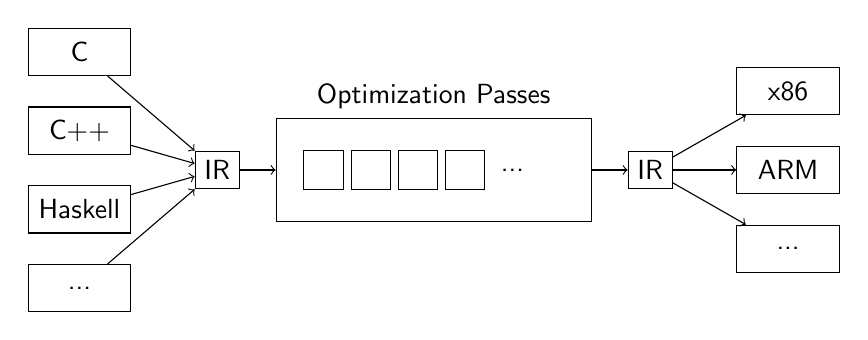
\begin{tikzpicture}
    \node[draw, minimum width=1.3cm, minimum height=0.6cm] at (-2.5,1.5) (C) {C};
    \node[draw, minimum width=1.3cm, minimum height=0.6cm] at (-2.5,0.5) (C++) {C++};
    \node[draw, minimum width=1.3cm, minimum height=0.6cm] at (-2.5, -0.5) (Haskell) {Haskell};
    \node[draw, minimum width=1.3cm, minimum height=0.6cm] at (-2.5, -1.5) (otherl) {...};
    \node[draw] at (-0.75, 0) (irl) {IR};
    
    \node[draw, label=Optimization Passes, minimum width=4cm, minimum height=1.3cm] at (2,0) (optimization) {};
    \node[draw, minimum size=0.5cm] at (0.6,0) {};
    \node[draw, minimum size=0.5cm] at (1.2,0) {};
    \node[draw, minimum size=0.5cm] at (1.8,0) {};
    \node[draw, minimum size=0.5cm] at (2.4,0) {};
    \node at (3.0, 0) {...};

    \node[draw] at (4.75, 0) (irr) {IR};
    \node[draw, minimum width=1.3cm, minimum height=0.6cm] at (6.5,1) (x86) {x86};
    \node[draw, minimum width=1.3cm, minimum height=0.6cm] at (6.5,0) (arm) {ARM};
    \node[draw, minimum width=1.3cm, minimum height=0.6cm] at (6.5,-1) (otherr) {...};

    \draw[->] (C) -- (irl);
    \draw[->] (C++) -- (irl);
    \draw[->] (Haskell) -- (irl);
    \draw[->] (otherl) -- (irl);

    \draw[->] (irl) -- (optimization);
    \draw[->] (optimization) -- (irr);

    \draw[->] (irr) -- (x86);
    \draw[->] (irr) -- (arm);
    \draw[->] (irr) -- (otherr);
  \end{tikzpicture}
  \caption{The general architecture of the \llvm{} compiler}
  \label{fig:llvm}
\end{figure}

\subsection{\qemu{}}
\qemu{} is a generic and open source machine emulator and visualizer.\cite{bellard2005qemu}
While it can be used as a full fledged virtualization environment and sandbox, all I need is its ability to run machine code for different architectures.
\qemu{} achieves high emulation speeds by changing the machine code of the emulated system (guest machine) into machine code that the running machine (host system) can understand, instead of simulating a guest machine CPU directly.
This translation is done by the Tiny Code Generator (TCG).
While this translation is exactly the opposite of what I would want, \qemu{} can be compiled with an optional filter called the TCG interpreter (TCI).
This interpreter runs all operations in on a simulated CPU, and thus allows me to examine the results for ``balancedness''.
Like using the \llvm{} compiler, using \qemu{} makes any evaluation mechanism I create for it applicable to desired target platform.

\section{Intended Methodology}
\label{sec:methodology}
aoeu

\section{Related Work}
\label{sec:related-work}
aoeu

\section{Possible Difficulties}
\label{sec:difficulties}
aoeu


\bibliographystyle{plain}
\bibliography{sources.bib}
\end{document}